\section{Уравнения механики деформируемого твёрдого тела}
\subsection{Уравнения механики сплошной среды в 1D}
\label{model-1d}
Рассмотрим уравнения МДТТ в случае одной пространственной переменной. Здесь $v$ -- скорость частиц среды, $\sigma$ -- напряжение, $E$ -- модуль Юнга, $\rho$ -- плотность вещества, $\varepsilon$ -- относительная деформация.

Запишем для частицы среды массой $dm$ и объёмом $S dx$ второй закон Ньютона
\begin{eqnarray}
dm \left(\frac{\partial v}{\partial t}\right)_{particle} = - \left(\sigma(x) - \sigma(x+dx)\right) S = 
\left(\frac{\partial \sigma}{\partial x}\right)_{t} S dx,
\end{eqnarray}
где $(\frac{\partial}{\partial t})_{particle}$ означает дифференцирование по времени в фиксированной частице, но не (!) фиксированной координате пространства,
\begin{eqnarray}
\rho\left(\frac{\partial v}{\partial t}\right)_{particle} = \left(\frac{\partial \sigma}{\partial x}\right)_{t} 
\label{newton}
\end{eqnarray}
и закон Гука
\begin{equation}
\varepsilon = \frac{\Delta_x(x+dx) - \Delta_x(x)}{dx} = 
\left(\frac{\partial \Delta_x}{\partial x}\right),
\end{equation}
где $\Delta_x$ -- малое отклонение частицы вещества от положения равновесия,
\begin{equation}
\sigma = E\left(\frac{\partial \Delta_x}{\partial x}\right).
\end{equation}
Производя дифференцирование по времени опять же в фиксированной частице вещества, получаем
\begin{equation}
\left(\frac{\partial \sigma}{\partial t}\right)_{particle} = E \left( \frac{\partial v}{\partial x} \right) _{t}.
\label{guk}
\end{equation}

Существуют два основных подхода к описанию движения сплошной среды \cite{sedov}:
\begin{itemize}
\item Эйлеров подход -- когда система координат (обозначим её $x$) выбирается жёстко связанной с неподвижным пространством
\item Лагранжев подход -- система координат ($\xi$) жёстко связана с самой средой ("вморожена" в неё в начальный момент времени, то есть фиксация $\xi$ есть не что иное, как фиксация частицы)
\end{itemize}
В этих системах уравнения движения имеют существенно разный вид, так как дифференцирования по времени при фиксированных $\xi$ и $x$ связаны соотношением для полной производной:
\begin{equation}
\left(\frac{\partial}{\partial t}\right)_{\xi} = \left(\frac{\partial}{\partial t}\right)_{x} + 
\left(\frac{\partial x}{\partial t}\right)_{\xi}\left(\frac{\partial}{\partial x}\right)_{t} =  \left(\frac{\partial}{\partial t}\right)_{x} + v_{\xi}\left(\frac{\partial}{\partial x}\right)_{t}
\end{equation}

Вводя вектор неизвестных $\vec{u} = (v, \sigma)^T$, перепишем \ref{newton} и \ref{guk} в виде
\begin{equation}
\left( \frac{\partial \vec{u}}{\partial t} \right) + \mathbf{A}\left( \frac{\partial \vec{u}}{\partial x} \right) = 0
\end{equation}

Наиболее простой вид матрица $\mathbf{A}$ имеет, когда производная по времени берётся при фиксированных  лагранжевых координатах (при этом $\frac{\partial \vec{u}}{\partial x}$ -- производная именно по неподвижным эйлеровым координатам):
\begin{displaymath}
\mathbf{A} =
\left( \begin{array}{cc}
0 & -\frac{1}{\rho} \\
-E & 0
\end{array} \right)
\end{displaymath}
В этих переменных уравнения являются линейными и не составляет сложности найти аналитическое решение переходом к инвариантам Римана $\vec{w}$\cite{vasyukov}. Решение представляется в виде двух волн, распространяющихся в разных направлениях с одинаковой постоянной скоростью $c = \sqrt{\frac{E}{\rho}}$:
\begin{equation}
\left\lbrace
\begin{array}{cc}
w_1(x,t) = w_1(x - ct,0)  \\
w_2(x,t) = w_2(x + ct,0),
\end{array}
\right.
\end{equation}
после чего осуществляется обратный переход к искомому вектору $\vec{u}$. Более подробно об этом в \ref{hyperbolic}.

В эйлеровых переменных в матрице $\mathbf{A}$ появляются диагональные конвективные члены, обусловленные переносом вещества:
\begin{displaymath}
\mathbf{A} =
\left( \begin{array}{cc}
v & -\frac{1}{\rho} \\
-E & v
\end{array} \right)
\end{displaymath} 
Они делают систему нелинейной. Аналитическое решение в общем случае не записывается. В каждый момент времени и в каждой точке пространства это две волны со скоростями $v(x,t) \pm c$. Из-за зависимости скоростей волн от скоростей частиц среды возможно формирование ударных волн, когда гладкое возмущение с течением времени переходит в разрывное.

В случае равенства одного из инвариантов Римана нулю получаем классическое одномерное квазилинейное уравнение. Решение формально можно записать в виде
\begin{equation}
w(x,t) = w(x - (c + v)t,0),
\label{quazilin}
\end{equation}
где $w$ -- не равный нулю инвариант. Так как здесь $v$ выражается через $w$, данное решение нельзя  непосредственно вычислить, но можно сколь угодно точно приблизить итерационным методом. 

Квазилинейные уравнения подробно рассмотрены в \cite{rogdestvenskiy}, откуда и были взяты вышеизложенные идеи.

\subsection{Уравнения движения и реологические соотношения в 3D}
Для математического моделирования волновых процессов в деформируемом твёрдом
теле используется система динамических уравнений \cite{sedov} в виде
\begin{eqnarray}
\label{rheology_equations}
\rho\dot{v}_i=\nabla_j\sigma_{ij}+f_i & \textrm{(уравнения движения)}\nonumber\\
\dot{\sigma}_{ij}=q_{ijkl}\dot{\varepsilon}_{kl}+F_{ij} & \textrm{(реологические
соотношения).}
\end{eqnarray}

Здесь $\rho$ – плотность среды, $v_i$ – компоненты скорости смещения,
$\sigma_{ij}$, $\varepsilon_{ij}$ -- компоненты тензоров напряжений и деформаций,
$\nabla_j$ – производная по $j$-й координате, $f_i$ – массовые
силы, действующие на единицу объёма, $F_{ij}$ -- силы, обусловленные вязкостью, $q_{ijkl}$ -- 
тензор упругих постоянных.

В случае малых деформаций тензор скоростей деформаций $e_{ij}=\dot{\varepsilon}_{ij}$ 
выражается через компоненты скорости смещения линейным образом:
\begin{equation}
e_{ij}=\frac{1}{2}(\nabla_j v_i+\nabla_i v_j).
\end{equation}

Вид компонент тензора 4-го порядка $q_{ijkl}$ определяется реологией среды. Для 
невязкого изотропного линейно-упругого материала
\begin{eqnarray}
\label{tensor_qijkl}
q_{ijkl}=\lambda\delta_{ij}\delta_{kl}+\mu(\delta_{ik}\delta_{jl}+\delta_{il}
\delta_{jk}) & \textrm {(изотропия)} \nonumber\\
F_{ij}=0 & \textrm {(отсутствует вязкость).}
\end{eqnarray}
В этом соотношении, которое обобщает закон Гука, $\lambda$ и $\mu$ -- параметры
Ляме, $\delta_{ij}$ -- символ Кронекера.

Для замыкания системы уравнений \ref{rheology_equations} её необходимо дополнить
уравнением состояния, определяющим зависимость плотности от напряжений:
например, $$\rho=const$$ или
$$\rho=\rho_0e^{\frac{p}{K}},$$
где $p=-\frac{1}{3}\sum\sigma_{kk}$ -- давление, $K=\lambda+\frac{2}{3}\mu$ --
коэффициент всестороннего сжатия.

\subsection{Модель пластического течения}
Существует большое количество феноменологических моделей пластической реологии сплошной среды.
Многие из них \cite{resler,kukudganov} основываются на критерии текучести $f(\sigma_{ij})$, определяющем переход между упругим $f(\sigma_{ij})<0$ и пластическим $f(\sigma_{ij})=0$ поведением материала. Случай $f(\sigma_{ij})>0$ полагается невозможным, то есть в пространстве напряжений компоненты $\sigma_{ij}$ не могут выйти за пределы поверхности, определяемой этим критерием. Это не означает, что напряжения не могут возрастать выше определённого предела, так как в процессе деформирования поверхность текучести может изменять свою форму и расширяться, как на рис. \ref{pic:uprochnenie}. Это называется упрочнением материала. Выделяют два основных вида упрочнения:
\begin{itemize}
\item Изотропное -- поверхность текучести расширяется симметрично относительно начала координат
\item Кинематическое -- поверхность текучести смещается без изменения формы
\end{itemize}
\begin{figure}[H]
\center{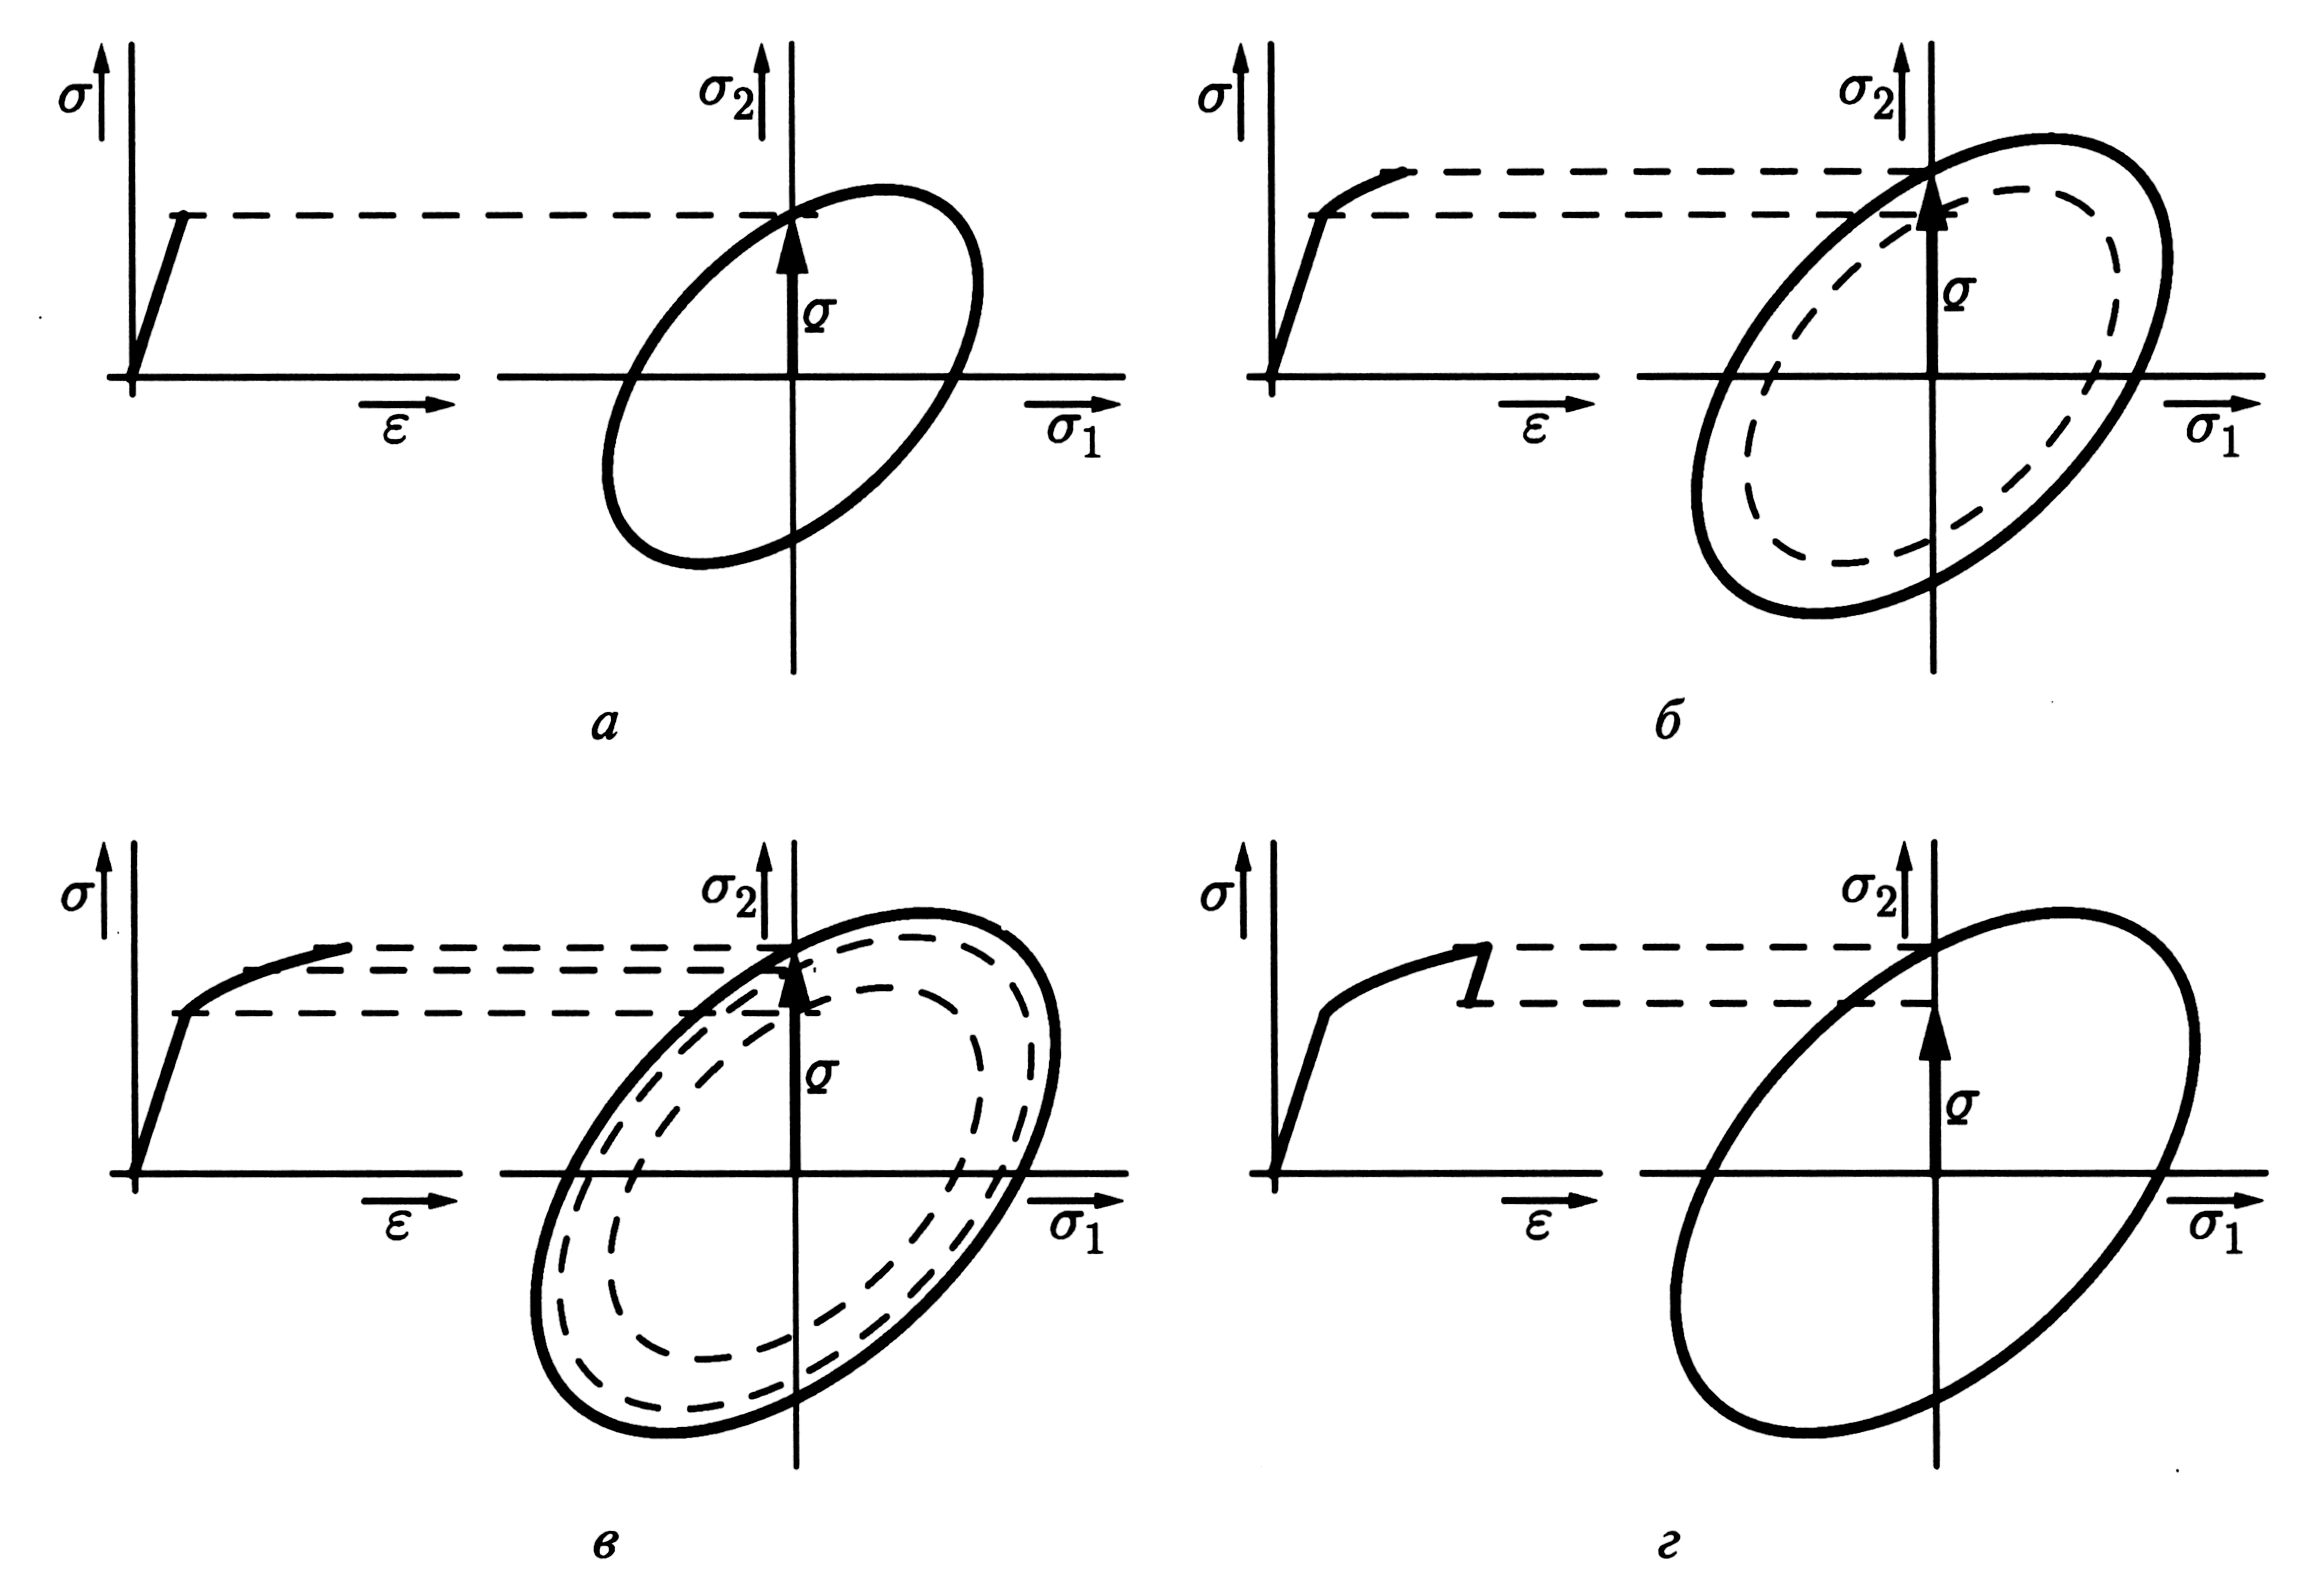
\includegraphics[width=0.75\textwidth]{png/3d/uprochnenie.png}}
\caption{Поверхность текучести и диаграмма $\varepsilon - \sigma$ для материала с изотропным упрочнением. а) Упругий участок, $f(\sigma_{ij})<0,$  б,в) Пластика, поверхность текучести расширяется с увеличением деформации, г) Разгрузка, остаточная деформация, поверхность текучести остаётся расширенной, область упругости увеличилась. Рисунок взят из \cite{resler}}
\label{pic:uprochnenie}
\end{figure}
Идеальнопластическим материалом, или материалом без упрочнения, называют среду с не меняющейся при деформациях функцией $f(\sigma_{ij})$. Диаграмма $\varepsilon - \sigma$ для такого материала представлена на рис. \ref{pic:eps-sigma}, a.

\begin{figure}[h!]
\begin{minipage}{0.47\linewidth}
\center{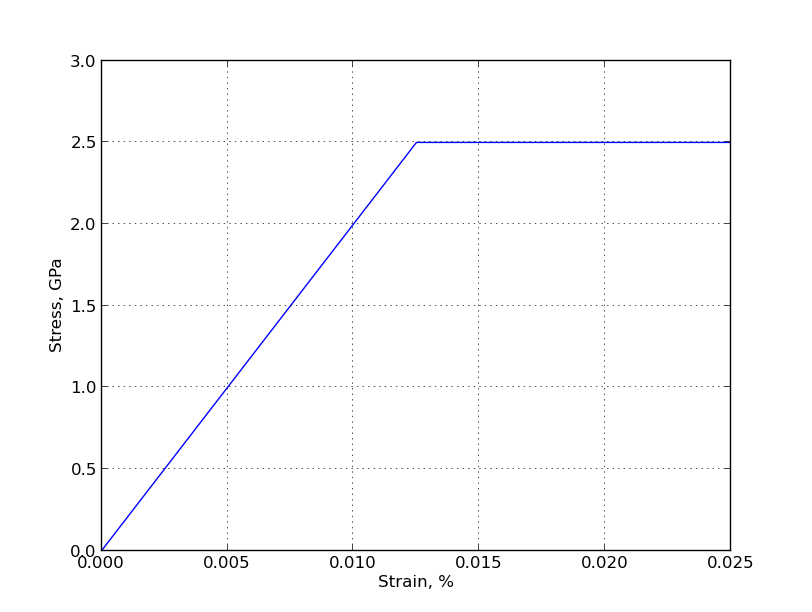
\includegraphics[width=1\linewidth]{png/1d/ideal-plastic.png}} a)
\end{minipage}
\begin{minipage}{0.47\linewidth}
\center{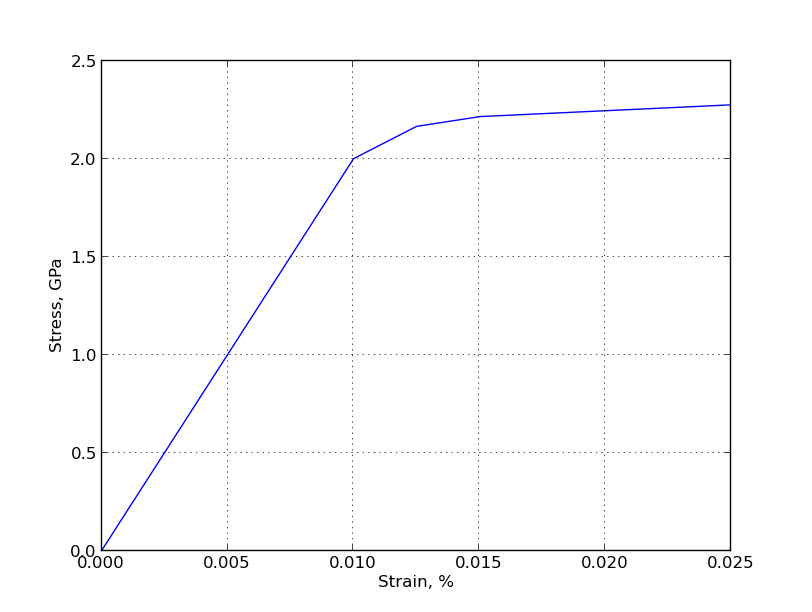
\includegraphics[width=1\linewidth]{png/1d/linear-plastic.png}} b)
\end{minipage}
\caption{Диаграмма $\varepsilon - \sigma$ для материалов a) без упрочнения, b) с кусочно-линейным упрочнением.}
\label{pic:eps-sigma}
\end{figure} 

\subsubsection{Критерий текучести Мизеса}
Для металлов установлено, что пластическая деформация обусловлена взаимным смещением кристаллических плоскостей и не изменяет объёма материала. Поэтому гидростатическое сжатие $$\sigma = \frac{\sigma_{ii}}{3}$$ не приводит к пластическим деформациям, и переход к пластике определяется только сдвиговыми напряжениями, то есть девиатором тензора напряжений: $$s_{ij} = \sigma_{ij} - \sigma\delta_{ij}.$$ Поэтому одним из широко используемых критериев является получаемая из инвариантов $s_{ij}$ функция
\begin{eqnarray}
\label{mizes}
f(\sigma_{ij}) = \frac{1}{2}s_{ij}s_{ji} - k^2_F
\end{eqnarray}

Получаемая поверхность текучести -- круговой цилиндр радиуса $k_F\sqrt{2}$ с осью $\sigma_1 = \sigma_2 = \sigma_3$ в пространстве главных напряжений. На рис.\ref{pic:mizes} приведён цилиндр и его сечение плоскостью $\sigma_3 = 0$.

\begin{figure}[h]
\center{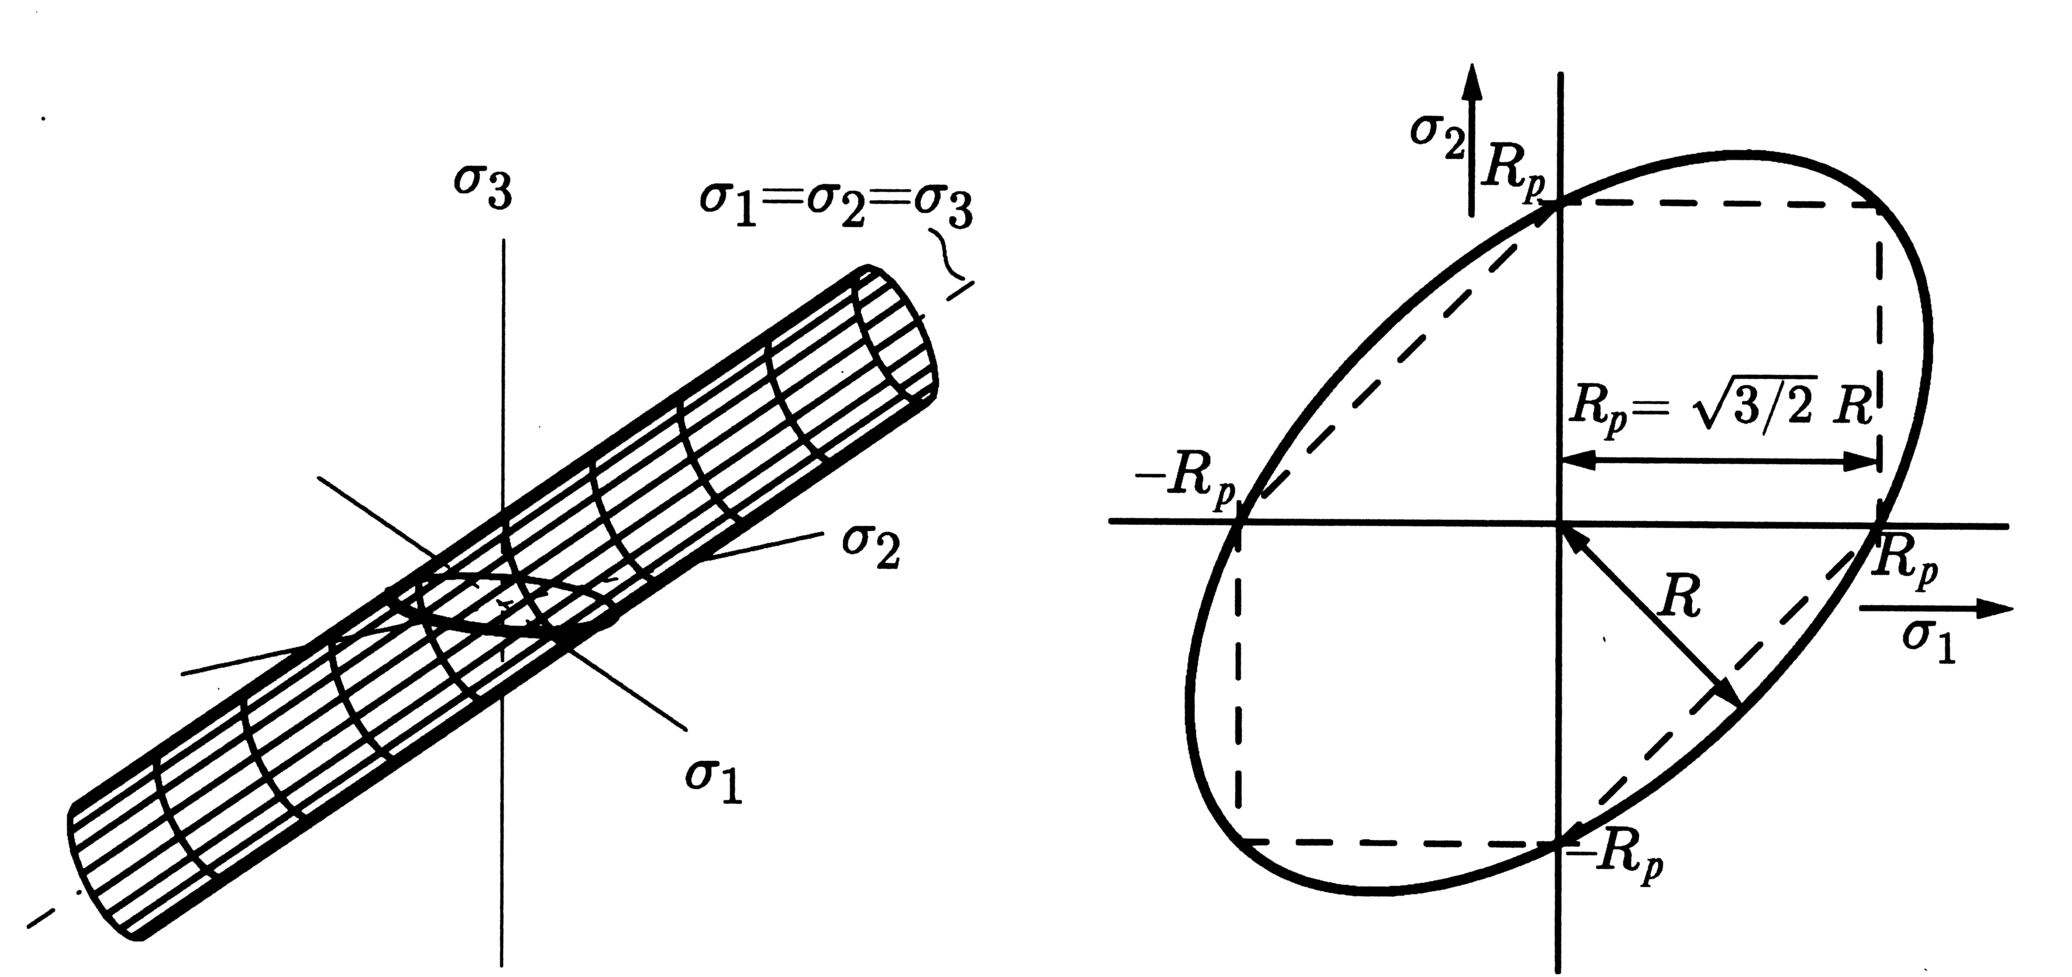
\includegraphics[width=\textwidth]{png/3d/mizes.png}}
\caption{Поверхность текучести в критерии Мизеса. Рисунок взят из \cite{resler}}
\label{pic:mizes}
\end{figure}

Для полимеров же величина предела текучести при сжатии и растяжении часто бывает различна. Поэтому в критерий текучести включаются слагаемые, зависящие от гидростатического давления, и соответствующая поверхность из цилиндрической переходит в параболическую (а) или коническую (б), как показано на рис.\ref{pic:plastic-tekuchest}.

\begin{figure}[h]
\center{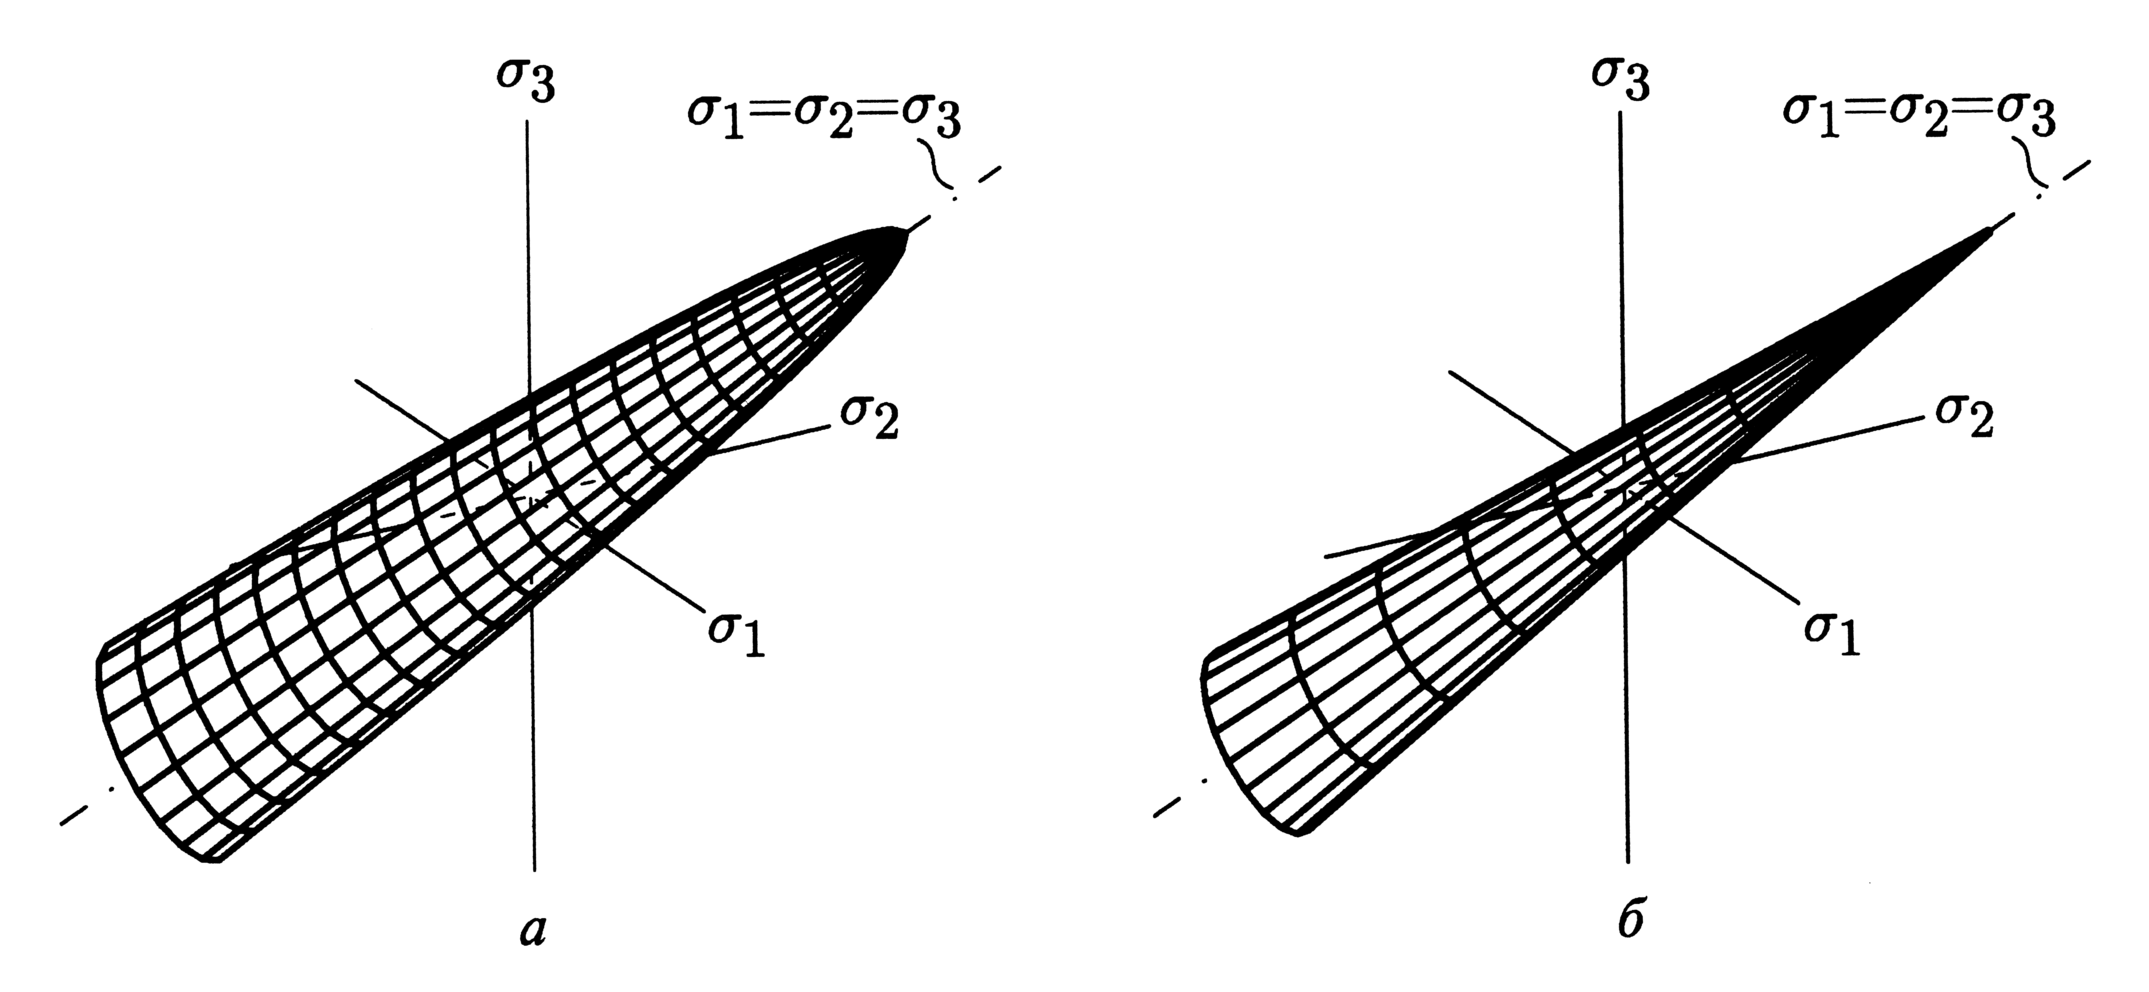
\includegraphics[width=\textwidth]{png/3d/plastic-tekuchest.png}}
\caption{Характерные поверхности текучести для пластиков. Рисунок взят из \cite{resler}}
\label{pic:plastic-tekuchest}
\end{figure}

В коде для 1D были испробованы модели с кусочно-линейным упрочнением. При одноосных деформациях такая модель сводится к ступенчатой зависимости модуля Юнга от напряжения (рис. \ref{pic:eps-sigma}, b). В коде для случая трёх измерений была реализована идеальнопластическая модель, то есть модель без упрочнения (рис. \ref{pic:eps-sigma}, a). 
 